\documentclass{uimppracticas}

%Permitir cabeceras y pie de páginas personalizados
\pagestyle{fancy}

%Path por defecto de las imágenes
\graphicspath{ {./images/} }

%Declarar formato de encabezado y pie de página de las páginas del documento
\fancypagestyle{doc}{
  %Pie de Página
  \footerpr{}{}{{\thepage} de \pageref{LastPage}}
}

%Declarar formato de encabezado y pie del título e indice
\fancypagestyle{titu}{%
  %Cabecera
  \headerpr{}{}{}
  %Pie de Página
  \footerpr{}{}{}
}

\appto\frontmatter{\pagestyle{titu}}
\appto\mainmatter{\pagestyle{doc}}

\begin{document}
	
%Comienzo formato título
\frontmatter

%Portada (Centrado todo)
\centeredtitle{./images/LogoUIMP.png}{Máster Universitario en Investigación en Inteligencia Artificial}{Curso 2020-2021}{Recuperación y extracción de información, \\ grafos y redes sociales}{Práctica Bloque II: Recuperación de información y minería de texto}

\begin{center}
\large \today
\end{center}

\vspace{40mm}

\begin{flushright}
 	{\bf Laura Rodríguez Navas}\\
 	\textbf{DNI:} 43630508Z\\
 	\textbf{e-mail:} \href{rodrigueznavas@posgrado.uimp.es}{rodrigueznavas@posgrado.uimp.es}
\end{flushright}

\newpage

%Índice
\tableofcontents

\newpage

%Comienzo formato documento general
\mainmatter

\setlength\parskip{2.5ex}

\section{Resumen}

En esta práctica se ha implementado un rastreador web (crawler) en Python~\cite{GitHubRepo} (ver sección~\ref{crawler}), que se complementa con un proceso de agrupamiento, también implementado en Python, de la información extraída de las páginas web que ha recopilado (ver sección~\ref{kmeans}). 

\section{Rastreador web (crawler)}\label{crawler}

En esta sección se describe como se ha implementado el rastreador web (crawler) en Python usando la librería \href{https://scrapy.org/}{Scrapy}. Para empezar con la implementación se debe ejecutar el siguiente comando:

\begin{lstlisting}[language=bash]
$ scrapy startproject books
\end{lstlisting}

Este comando crea un proyecto Scrapy en el directorio books, siguiendo la \href{https://docs.scrapy.org/en/latest/topics/commands.html#default-structure-of-scrapy-projects}{estructura por defecto} común para todos los proyectos Scrapy, y el fichero \textit{scrapy.cfg} que contiene el nombre del módulo de Python que define la configuración del proyecto books (\textit{books.settings}). El proyecto lo he nombrado books, porqué se rastreará el catálogo de libros que se encuentra en la página web: \url{http://books.toscrape.com}.

Una vez se ha creado el proyecto, se definen los ítems de cada libro que se quieren extraer del catálogo. En este caso los ítems que se van a extraer son: el título, la categoría, la descripción, el precio y la valoración de cada libro. Para ello, se tiene que modificar el fichero \textit{books/items.py}, para incluir los cinco ítems que se quieren extraer. Vemos el contenido de \textit{items.py} a continuación:

\begin{lstlisting}[language=python]
import scrapy


class BooksItem(scrapy.Item):
	# define the fields for your item here like:
	# name = scrapy.Field()
	title = scrapy.Field()
	category = scrapy.Field()
	description = scrapy.Field()
	price = scrapy.Field()
	rating = scrapy.Field()
\end{lstlisting}

El siguiente paso es describir la manera de extraer la información definida en el fichero \textit{items.py}. Para ello, se utilizarán reglas de expresión \href{https://www.w3.org/TR/xpath/all/}{XPath} y \href{https://www.w3.org/TR/selectors/}{CSS}. Por ejemplo, si nos fijamos en el código HTML de uno de los libros que se van rastrear (ver Figura \ref{book}), veremos que el título del libro es fácil de extraer con la siguiente regla de expresión CSS: \textbf{"h1 ::text"}. Cuando la extracción de información se complica un poco más, se usan reglas de expresión XPath. Por ejemplo, para extraer las descripciones de todos los libros se usará la regla de expresión: \textbf{"//div[@id='product\_description']/following-sibling::p/text()"}. Una vez, definidas todas las reglas de expresión para cada ítem que se va a rastrear, se crea la araña \textit{books/spiders/books\_toscrape.py}.

Las arañas son clases que definen cómo se rastrea una página web determinada (o un grupo de páginas web), incluido cómo realizar el rastreo y cómo extraer la información deseada. En otras palabras, las arañas son el lugar donde se define el comportamiento personalizado para rastrear y analizar las páginas web. En el caso de la práctica, en la araña \textit{books.toscrape} será el lugar donde se definen las reglas de expresión. En las arañas también se tienen que especificar las solicitudes iniciales para rastrear las URLs y una función de devolución de llamada (\textit{parse}) a la que se llamará para generar los ítems de respuesta de esas solicitudes. Por último, los ítems devueltos por las arañas normalmente se conservan en una base de datos o se escriben en un archivo. En el caso de la práctica, en la araña \textit{books.toscrape}, los ítems (título, categoría, descripción, precio y valoración de cada libro) serán guardados en el fichero \textit{books.json}. Esta araña que procesa todas las URLs descubiertas de la \href{http://books.toscrape.com}{práctica} utilizando la función \textit{parse}, que a su vez llama a la función \textit{parse\_book\_page} donde son definidas todas las reglas de expresión de cómo extraer la información deseada, se muestra a continuación:

\begin{lstlisting}[language=python]
import scrapy


class BooksToscrapeSpider(scrapy.Spider):
	name = 'books.toscrape'
	allowed_domains = ['books.toscrape.com']
	start_urls = ['http://books.toscrape.com/']
	
	def parse(self, response):
		for book_url in response.css("article.product_pod > h3 > a ::attr(href)").extract():
			yield scrapy.Request(response.urljoin(book_url), callback=self.parse_book_page)
		next_page = response.css("li.next > a ::attr(href)").extract_first()
		if next_page:
			yield scrapy.Request(response.urljoin(next_page), callback=self.parse)
	
	@staticmethod
	def parse_book_page(response):
		item = {}
		product = response.css("div.product_main")
		item["title"] = product.css("h1 ::text").extract_first()
		item['category'] = response.xpath("//ul[@class='breadcrumb']/li[@class='active']/preceding-sibling::li[1]/a/text()").extract_first()
		item['description'] = response.xpath("//div[@id='product_description']/following-sibling::p/text()").extract_first()
		price = response.xpath('//th[text()="Price (incl. tax)"]/following-sibling::td/text()').extract_first()
		item['price'] = price.replace('£', '')
		rating = response.xpath('//*[contains(@class, "star-rating")]/@class').extract_first()
		item['rating'] = rating.replace('star-rating ', '')
		yield item
\end{lstlisting}

En este momento ya se puede iniciar la araña, pero primero es recomendable modificar el fichero \textit{books/settings.py} para limitar el acceso de la araña al catálogo web, ya que podemos generar un ataque \href{https://es.wikipedia.org/wiki/Ataque_de_denegaci%C3%B3n_de_servicio}{DDoS}. Para ello, debemos descomentar la variable \href{https://docs.scrapy.org/en/latest/topics/settings.html#download-delay}{DOWNLOAD\_DELAY} y darle un valor en segundos (p.ej. DOWNLOAD\_DELAY = 3). 	
	
\begin{figure}[h]
	\centering
	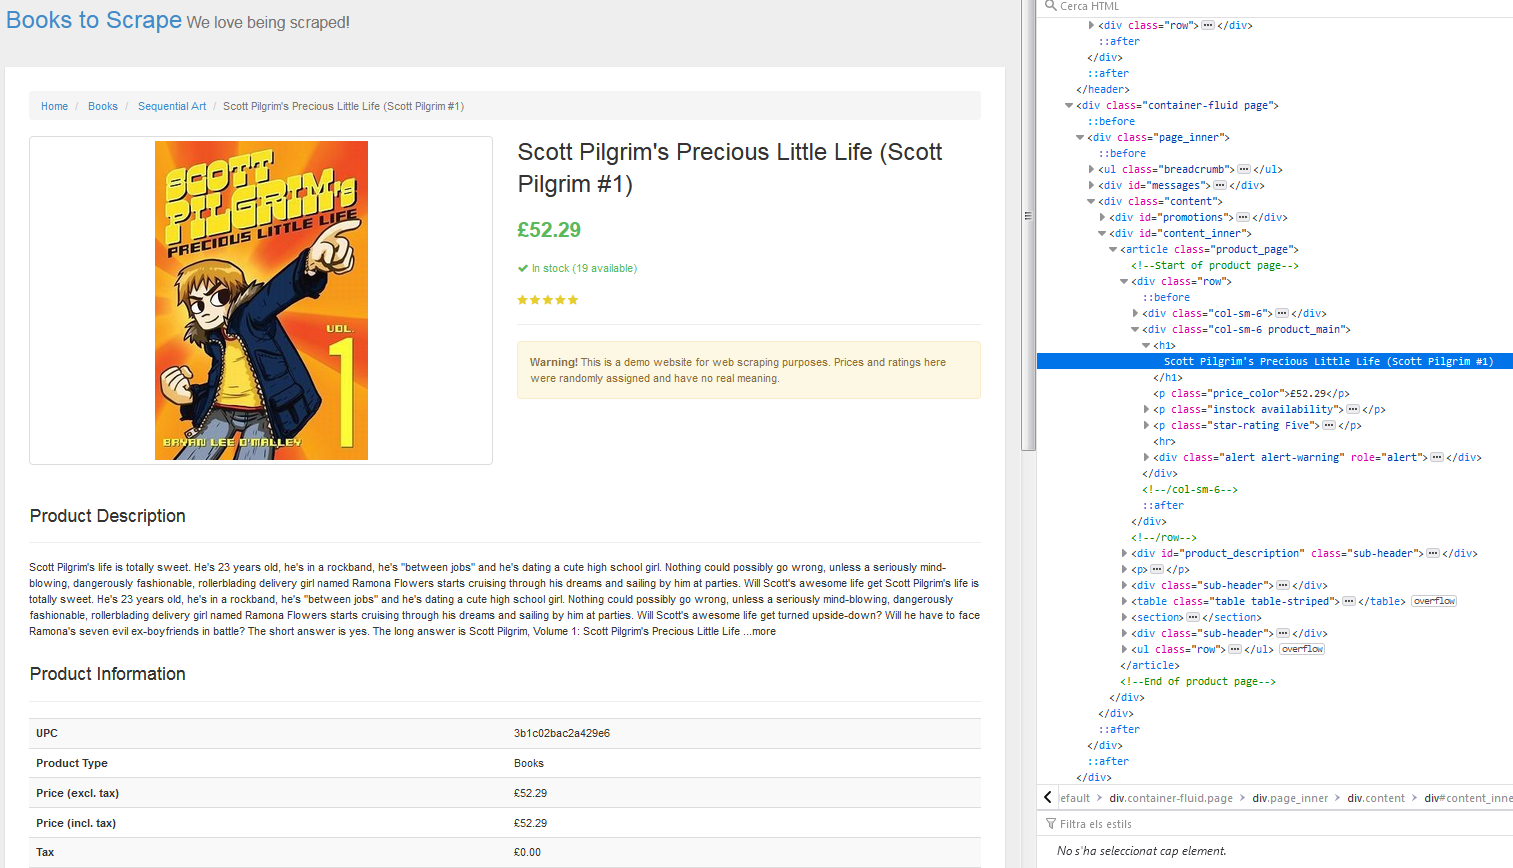
\includegraphics[scale=0.35]{images/book}
	\caption{Ejemplo de libro a rastrear.}
	\label{book}
\end{figure}

Finalmente, ya podemos iniciar la araña para que recupere la información del catálogo y la guarde en el fichero \textit{books.json}:

\begin{lstlisting}[language=bash]
	$ cd books
	$ scrapy crawl books.toscrape -o books.json
\end{lstlisting}

\section{K-Means}\label{kmeans} 

En esta sección se describe como se ha implementado el proceso de agrupamiento en Python (ver directorio kmeans en~\cite{GitHubRepo}) usando la librería scikit-learn~\cite{scikit-learn}. Existen muchos algoritmos de agrupación, y para esta práctica se ha elegido el algoritmo \href{https://scikit-learn.org/stable/modules/generated/sklearn.cluster.KMeans.html}{K-Means}. Concretamente, el algoritmo K-Means agrupará los títulos de los libros del catálogo web (recuperados en la sección~\ref{crawler}) en diferentes clústeres.

\subsection{Datos de entrada para K-Means}

Si nos fijamos en el fichero \textit{kmeans/kmeans.py}, vemos que empieza extrayendo la información de los libros almacenada en el fichero \textit{books/books.json}, que contiene 1000 documentos, y la convierte en un \textit{DataFrame}. Después se eliminan los valores NaN que pudieran existir en él y también es almacenado en un fichero CSV. Para ello, se usa la librería pandas~\cite{jeff_reback_2020_4309786}.

\begin{lstlisting}[language=python]
# create df
books = open("../books/books.json", "r")
dict_books = json.load(books)
df = pd.DataFrame.from_dict(dict_books)

# remove null values from df
df = df.dropna()

# save df to csv
df.to_csv("books.csv", index=False, sep=",")
\end{lstlisting}

\begin{definition}
Un DataFrame es una estructura de datos bidimensional etiquetada que acepta diferentes tipos datos de entrada organizados en columnas. Se puede pensar en un DataFrame como una hoja de cálculo o una tabla SQL.
\end{definition}

Las diez primeras líneas que forman el conjunto de datos de entrada:

\begin{figure}[h]
	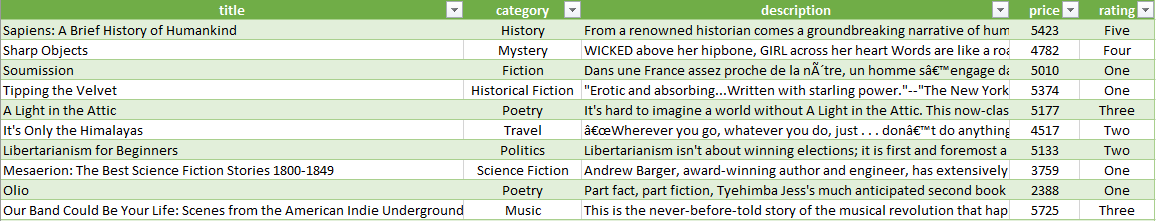
\includegraphics[scale=0.55]{images/data}
	\caption{Primeras líneas del conjunto de datos de entrada.}
	\label{data}
\end{figure}

\subsection{Extracción de características}

Para cada título del conjunto de datos, calcularemos los valores de \href{https://es.wikipedia.org/wiki/Tf-idf}{TF-IDF}.

\begin{lstlisting}[language=python]
vec = TfidfVectorizer(stop_words='english')
vec.fit(df['title'])
features = vec.transform(df['title'])
\end{lstlisting}

Ahora que tenemos la matriz de características, podemos enviarla al modelo para el entrenamiento.

\subsection{Entrenamiento del algoritmo}

\subsection{Visualización}

\renewcommand{\refname}{Bibliografía}
\bibliographystyle{unsrt}
\bibliography{biblio}

\end{document}
